
In this chapter we reinterpret modular forms as functions on certain very interesting geometric objects.

\section{Lattices and tori}
\begin{definition}
  A \emphh{lattice} is a free $\ZZ$-module $\Lambda$ of rank $2$ inside $\CC$ which contains an $\RR$-basis for $\CC$. Concretely, $\Lambda = \ZZ\omega_1\oplus \ZZ\omega_2$, where $\omega_1$ and $\omega_2$ are $\RR$-linearly independent complex numbers. We will always assume that $\omega_1/\omega_2\in\HH$, which can always be accomplished by possible swapping them.
\end{definition}

As you know, in general there are many choices for a basis of a given submodule.
\begin{proposition}
\label{prop:nine}
  Suppose that $\Lambda=\langle \omega_1,\omega_2\rangle$ and $\Lambda'=\langle \omega_1',\omega_2'\rangle$. Then $\Lambda = \Lambda'$ if and only if there exists $\gamma\in\SL_2(\ZZ)$ such that
\[
\mat{\omega_1\\\omega_2} = \gamma\mat{\omega'_1\\\omega'_2}.
\]
\end{proposition}
\begin{proof}
  Exercise.
\end{proof}

Lattices become interesting when we quotient $\CC$ out by them.
\begin{definition}
  A \emphh{complex torus} is the set $\CC/\Lambda =\{z+\Lambda~|~ z\in\CC\}$. It has the structure of an abelian group, and analytically it is a torus (a genus one Riemann surface).
\end{definition}
\begin{figure}
\begin{center}
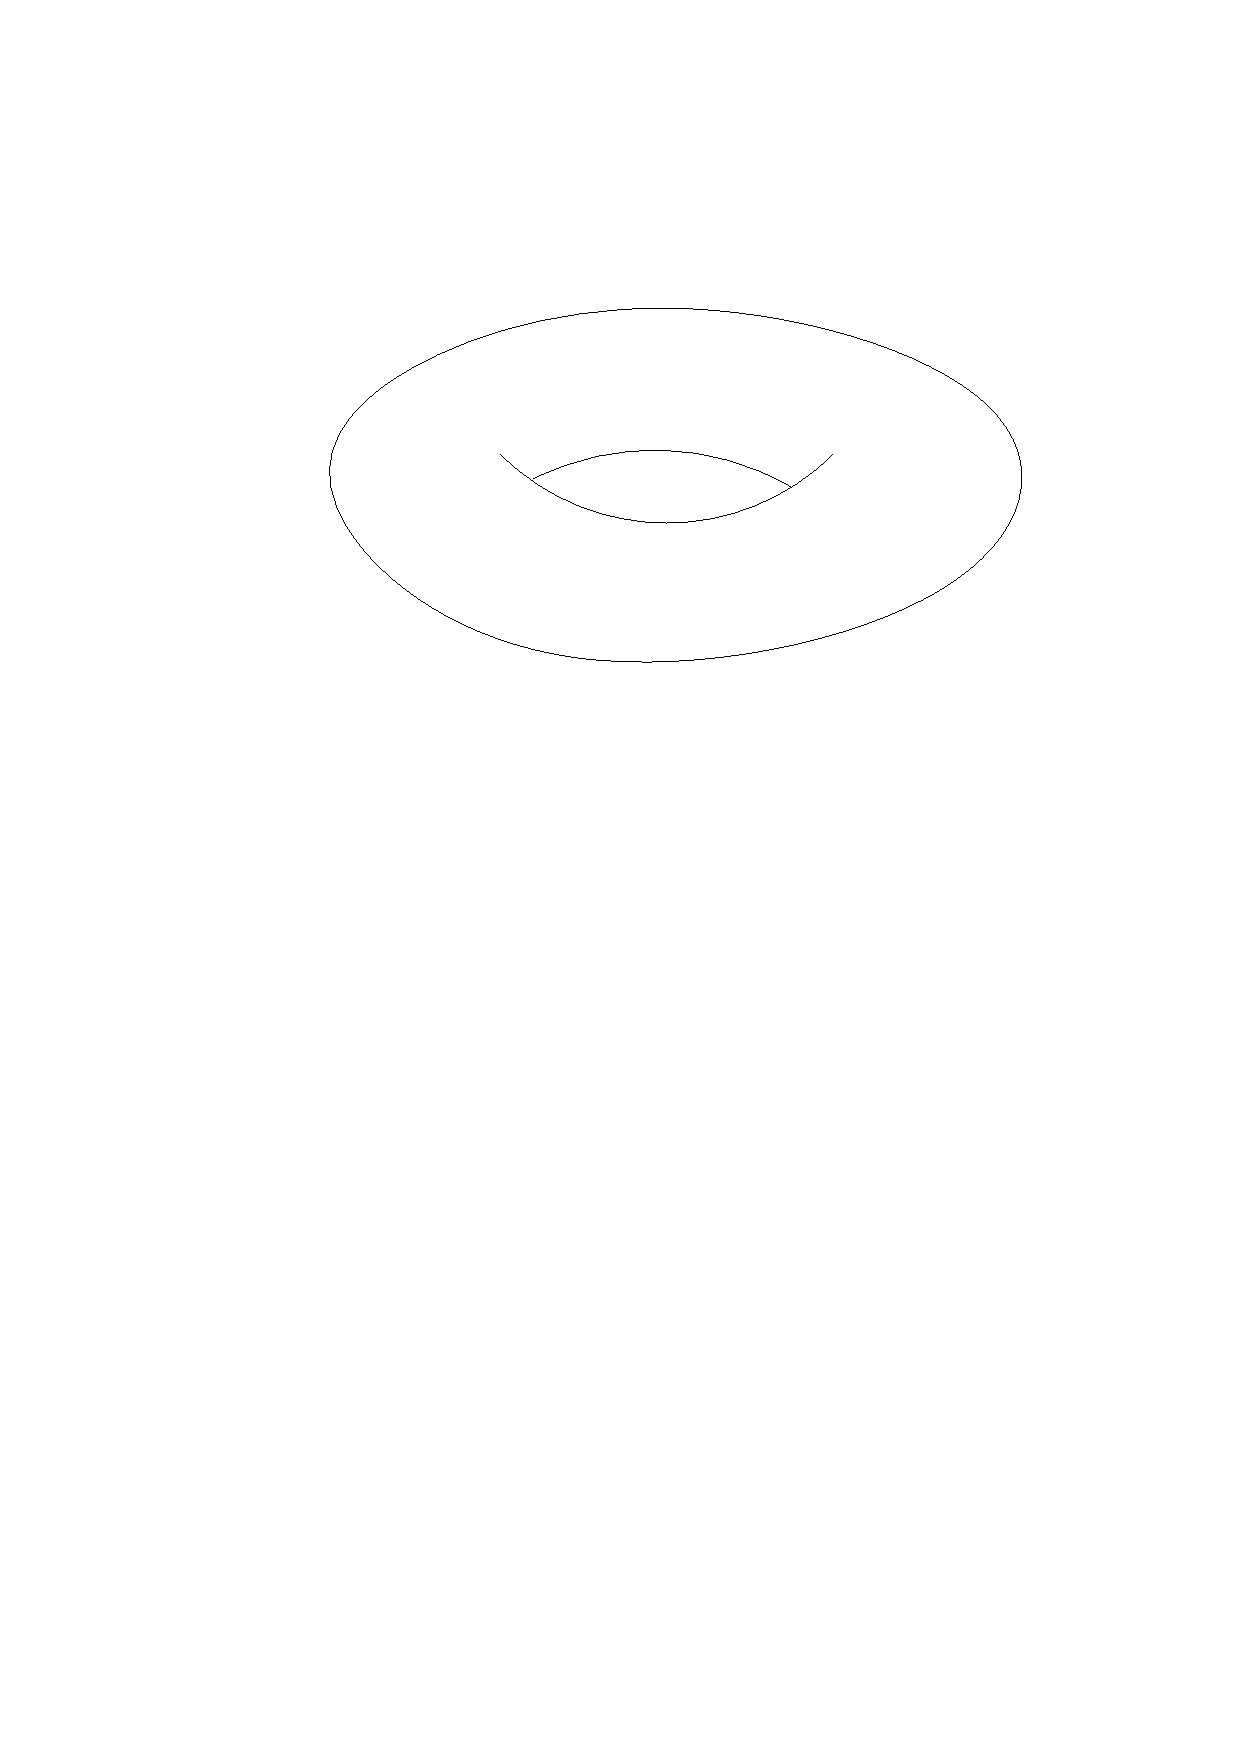
\includegraphics[height=3cm]{torus.pdf}
\end{center}
\label{fig:torus}
\end{figure}
\begin{proposition}
  Suppose that $\varphi\colon\CC/\Lambda\to\CC/\Lambda'$ is a holomorphic map. Then there exist complex numbers $m$ and $b$ such that:
  \begin{enumerate}
  \item $m\Lambda\subseteq \Lambda'$, and
  \item $\varphi(z+\Lambda)=mz+b+\Lambda'$.
  \end{enumerate}
Moreover, $\varphi$ is invertible if and only if $m\Lambda=\Lambda'$.
\end{proposition}
\begin{proof}
 The complex plane $\CC$ is the universal covering space of $\CC/\Lambda$ and $\CC/\Lambda'$. Therefore, $\varphi$ can be lifted to a map $\tilde\varphi\colon\CC\to\CC$. Suppose now that $\lambda\in\Lambda$, and define
\[
f_\lambda(z)=\tilde\varphi(z+\lambda)-\tilde\varphi(z).
\]
\begin{figure}[h]
  \centering
  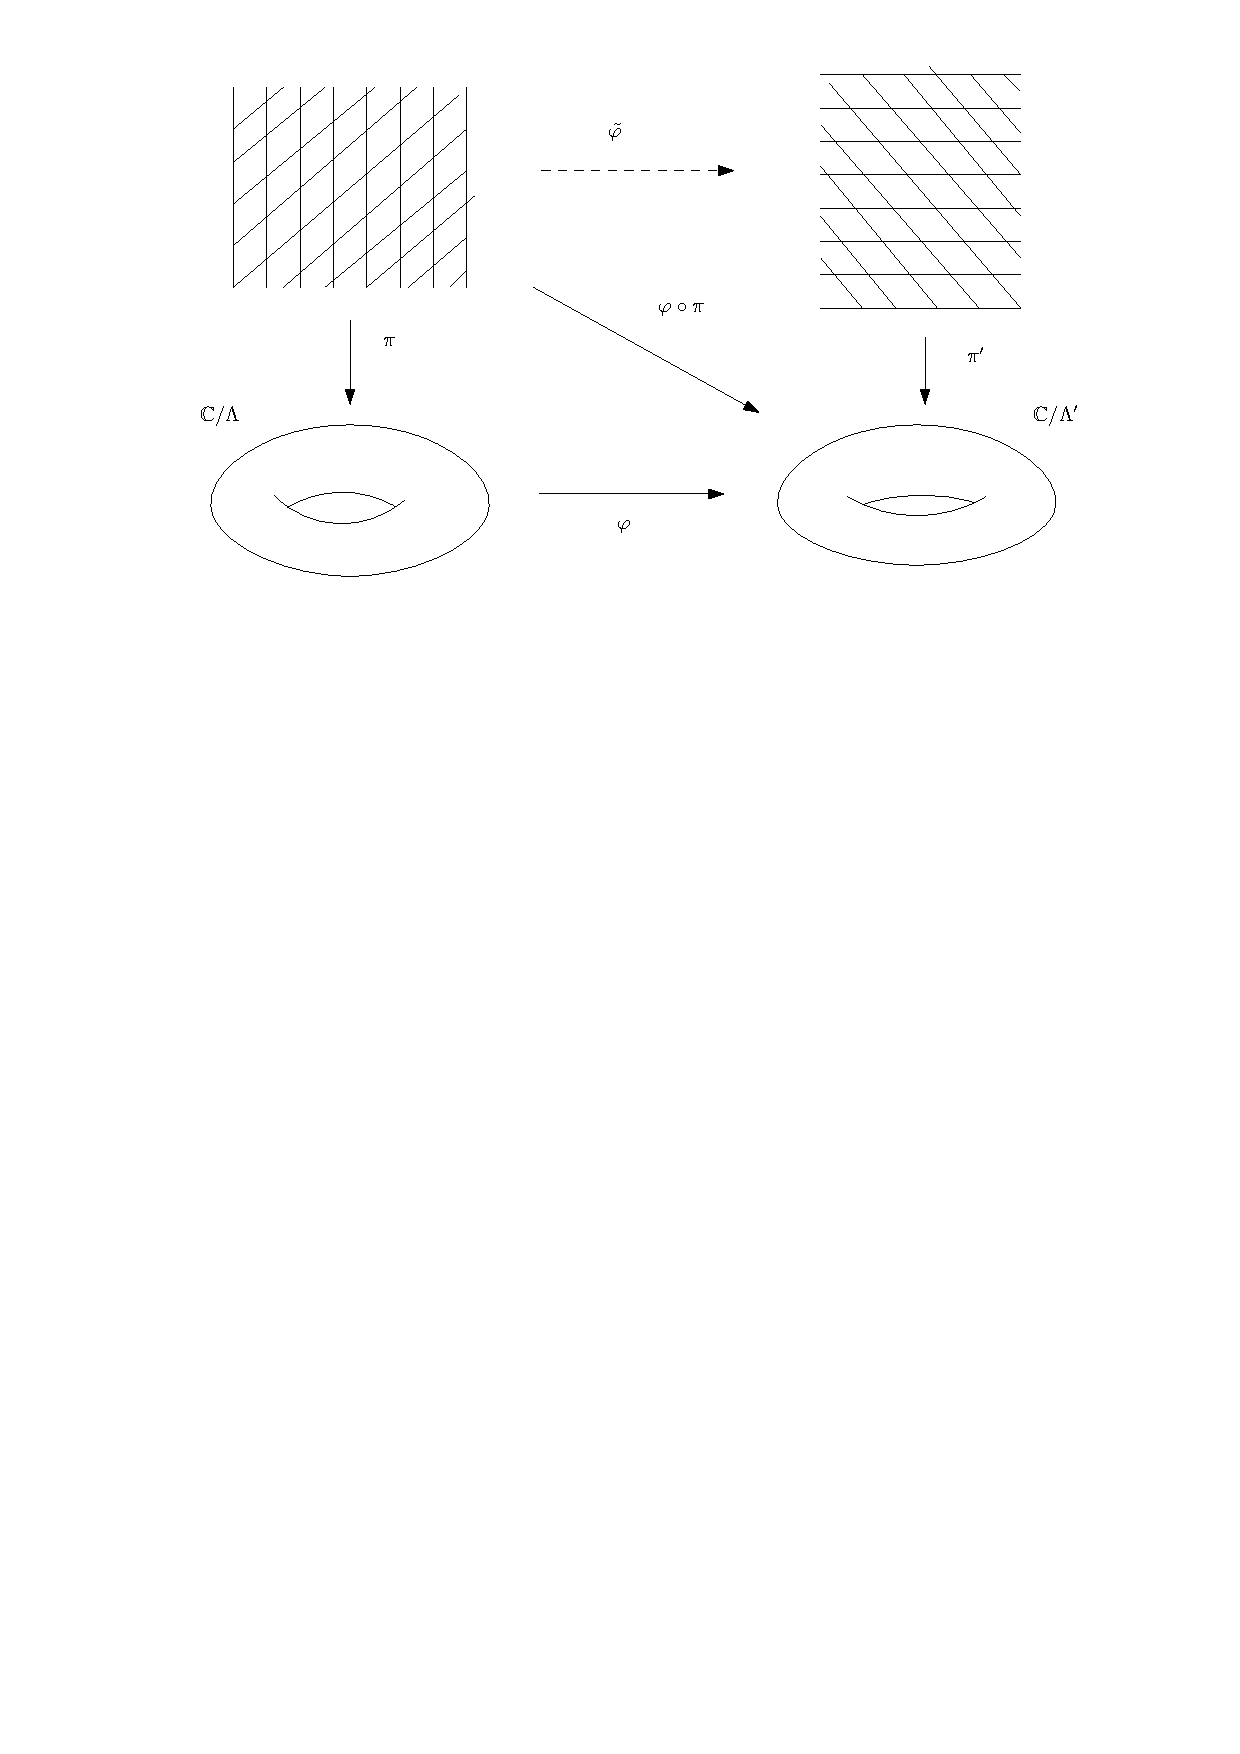
\includegraphics[height=5cm]{Pictures/universal_covering_space.pdf}

  \caption{Lifting to the universal covering space}
  \label{fig:universal-covering-space}
\end{figure}
Then $f_\lambda$ is continuous and has image in $\Lambda'$. Since $\Lambda'$ is discrete, necessarily $f_\lambda$ is constant. Consider the derivative. For each $\lambda\in\Lambda$, we have
\[
\tilde\varphi'(z+\lambda)=\tilde\varphi'(z).
\]
Therefore $\tilde\varphi'(z)$ is holomorphic and doubly-periodic, hence bounded. By Liouville's theorem, $\tilde\varphi'$ is constant. We deduce that $\tilde\varphi(z)=mz+b$, as wanted.
\end{proof}

\begin{corollary}
  Let $\varphi\colon\CC/\Lambda\to\CC/\Lambda'$ be a holomorphic map. Then $\varphi$ is a group homomorphism if and only if $\varphi(0)=0$, if and only if $b\in\Lambda'$.
\end{corollary}

\begin{remark}
  If $\varphi$ as above is a holomorphic group isomorphism, then necessarily $m\Lambda=\Lambda'$ and also $\varphi(z+\Lambda)=mz+\Lambda'$.
\end{remark}

Here are two examples of possible maps like the ones above.
\begin{example}
  The map \emphh{multiplication-by-$N$}, usually written $[N]$, is a homomorphism:
\[
\xymatrix@R5pt{\CC/\Lambda\ar[r]^{[N]}&\CC/\Lambda\\
z+\Lambda\ar@{|->}[r]&Nz+\Lambda
}
\]
The kernel of $[N]$ is the group of $N$-torsion points, isomorphic to $\ZZ/N\ZZ\times\ZZ/N\ZZ$.
\end{example}

\begin{example}
  Consider $\Lambda=\ZZ\omega_1\oplus\ZZ\omega_2$. Define $\tau=\omega_1/\omega_2\in \HH$, and set $\Lambda_\tau=\ZZ\tau\oplus\ZZ$. Then $\CC/\Lambda\cong \CC/\Lambda_\tau$.
\end{example}

The previous example can be brought a little bit further as follows.
\begin{lemma}
  The complex tori $\CC/\Lambda_\tau$ and $\CC/\Lambda_{\tau'}$ are isomorphic if and only if $\tau=\gamma\tau'$ for some $\gamma\in\SL_2(\ZZ)$.
\end{lemma}
\begin{proof}
  Suppose that
\[
\tau=\gamma\tau'=\frac{a\tau'+b}{c\tau'+d}.
\]
Let $m=c\tau'+d$. Then $m\Lambda_\tau = \ZZ(a\tau'+b)\oplus\ZZ(c\tau'+d)$. By Proposition~\ref{prop:nine}, this lattice is the same as $\ZZ\tau'\oplus\ZZ=\Lambda_{\tau'}$. The other direction is obtained by reading the equalities in reverse.
\end{proof}
\begin{remark}
  We have just seen that there is a ``natural bijection'' between isomorphism classes of tori and elements $\tau\in\SL_2(\ZZ)\backslash\HH$. This innocent statement is \textbf{really} important.
\end{remark}

\begin{example}[Eisenstein series attached to a lattice]
  Let $\Lambda$ be a lattice. Define, for $k>2$ even,
\[
G_k(\Lambda)=\sumprime_{\omega\in\Lambda}\omega^{-k}.
\]
Note that $G_k(\Lambda_\tau) = G_k(\tau)$ is the usual Eisenstein series defined in the previous chapter. The transformation law reads in this case:
\[
G_k(m\Lambda)=m^{-k}G_k(\Lambda).
\]
\end{example}
\section{Tori and elliptic curves}
The next goal is to relate $\CC/\Lambda$ to elliptic curves. This will allow to think of modular forms as functions either on lattices or on elliptic curves.

\subsection{Meromorphic functions on \texorpdfstring{$\CC/\Lambda$}{C/L}}
\label{sec:meromorphic-functions-CmodLambda}

Let $\CC(\Lambda)$ be the field of meromorphic functions on $\CC/\Lambda$. That is, meromorphic functions $f\colon\CC\to\CC$ satisfying $f(z+\lambda)=f(z)$ for all $\lambda\in\Lambda$.
\begin{proposition}
  Let $f\in\CC(\Lambda)$. Then:
  \begin{enumerate}
  \item $\sum_{z\in\CC/\Lambda} \res_z f = 0$.
  \item $\sum_{z\in\CC/\Lambda} \ord_z f = 0$.
  \item $\sum_{z\in\CC/\Lambda} z\ord_z f\in\Lambda$.
  \end{enumerate}
\end{proposition}
\begin{proof}
  Consider a fundamental parallelepiped $D$ which misses all zeroes and poles. This can be done because zeroes and poles form a discrete set. Now one can compute the quantities
\[
\frac{1}{2\pi i} \int_{\partial D} f(z)dz,\quad \frac{1}{2\pi i} \int_{\partial D} \frac{f'(z)}{f(z)}dz\quad, \text{and }\frac{1}{2\pi i} \int_{\partial D} \frac{zf'(z)}{f(z)}dz.
\]
\end{proof}
\begin{definition}
  The \emphh{order of a meromorphic function} $f$ is the number $\ord(f)$ of zeroes (which equals the number of poles) of $f$, when counted with multiplicities.
\end{definition}
Note that the first statement in the above proposition implies that $\ord(f)\geq 2$.

\subsection{The Weierstrass \texorpdfstring{$\wp$}{P}-function}
\label{sec:weierstrass-pe}

Consider the following function:
\[
\wp_\Lambda(z)=\frac{1}{z^2}+\sumprime_{w\in\Lambda} \left(\frac{1}{(z-w)^2} - \frac{1}{w^2}\right).
\]
It is immediate to see that $\wp_\Lambda$ is an even function, which converges absolutely and uniformly on compact sets away from $\Lambda$.
\begin{lemma}
  The function $\wp_\Lambda$ is $\Lambda$-periodic.
\end{lemma}
\begin{proof}
  Note that the derivative of $\wp_\Lambda$ is
\[
\wp_\lambda'(z)=-2\sum_{w\in\Lambda} \frac{1}{(z-w)^3},
\]
which is clearly $\Lambda$-periodic. Set $f(z)=\wp_\Lambda(z+w_1)-\wp_\Lambda(z)$, where $w_1\in\Lambda$. Then $f'(z)=0$, so $f$ is constant, say $f(z)=c$. To determine $c$, set $z=-\frac{w}{2}$ and note that since $\wp_\Lambda$ is even, we get
\[
c=\wp_\Lambda(w_1/2)-\wp_\Lambda(-w_1/2) = 0.
\]
Therefore $f(z)=0$, and thus $\wp_\Lambda$ is $\Lambda$-periodic.
\end{proof}

The lemma gives that $\wp_\lambda(z)$ belongs to $\CC(\Lambda)$. In fact, $\CC(\Lambda)$ is generated by $\wp_\Lambda$ and $\wp'_\Lambda$, but we are not going to prove this here.

\begin{proposition}
  The Laurent expansion of $\wp_\Lambda(z)$ at $z=0$ is
\[
\wp_\Lambda(z) = \frac{1}{z^2} + \sum_{n\geq 2,\text{ even}} (n+1)G_{n+2}(\Lambda)z^{n},
\]
and it has radius of convergence equal to the lattice point closest to the origin.
\end{proposition}
\begin{proof}
  See~\cite[Proposition 1.4.1]{diamond-shurman}.
\end{proof}

These expansions allow us to find algebraic relations between $\wp_\Lambda$ and $\wp'_\Lambda$. Since
\[
\wp_\Lambda = \frac{1}{z^2}+3G_4(\Lambda)z^2+O(z^4)
\]
and
\[
\wp'_\Lambda = \frac{-2}{z^3} + 6G_4(\Lambda)z + O(z^3),
\]
we deduce:
\[
(\wp_\Lambda')^2=\frac{4}{z^6}+O(z^{-2}) = 4(\wp_\Lambda)^3 + O(z^{-2}).
\]
We can work with a couple more terms of the expansions, to get:
\[
(\wp_\Lambda')^2 = 4(\wp_\Lambda)^3-60G_4(\Lambda)\wp_\Lambda-140G_6(\Lambda)+F(z),\quad F(z)=O(z^2).
\]
Finally, note that $F(z)$ is $\Lambda$-periodic so by Liouville's theorem it must be constant $0$.

\begin{proposition}
  Let $g_2(\Lambda) = 60G_4(\Lambda)$ and $g_3(\Lambda)=140G_6(\Lambda)$. Then:
  \begin{enumerate}
  \item The point $(\wp_\Lambda(z),\wp'_\Lambda(z))$ lies on the elliptic curve
\[
E_\Lambda\colon Y^2=4X^3-g_2(\Lambda)X-g_3(\Lambda).
\]
\item $E_\Lambda$ can be written as $Y^2=4(X-e_1)(X-e_2)(X-e_3)$, where
\[
e_i = \wp_\Lambda(w_i/2),\quad w_3 = w_1+w_2.
\]
Moreover, this equation is nonsingular (that is, the $e_i$ are all distinct).
  \end{enumerate}
\end{proposition}

\begin{proof}
  It only remains to prove the second statement. Since $\wp_\Lambda'$ is odd and periodic, we get:
\[
\wp_\Lambda'(w_i/2) = \wp_\Lambda'(-w_i/2) = -\wp_\Lambda'(w_i/2),
\]
so $\wp_\Lambda'(w_i/2)$ is $0$. Since $\wp_\Lambda$ takes the value $e_i$ twice and $\wp_\Lambda$ has degree $2$, it does not take the value $e_i$ at any other points outside the $2$-torsion.
\end{proof}

\begin{figure}
  \centering
  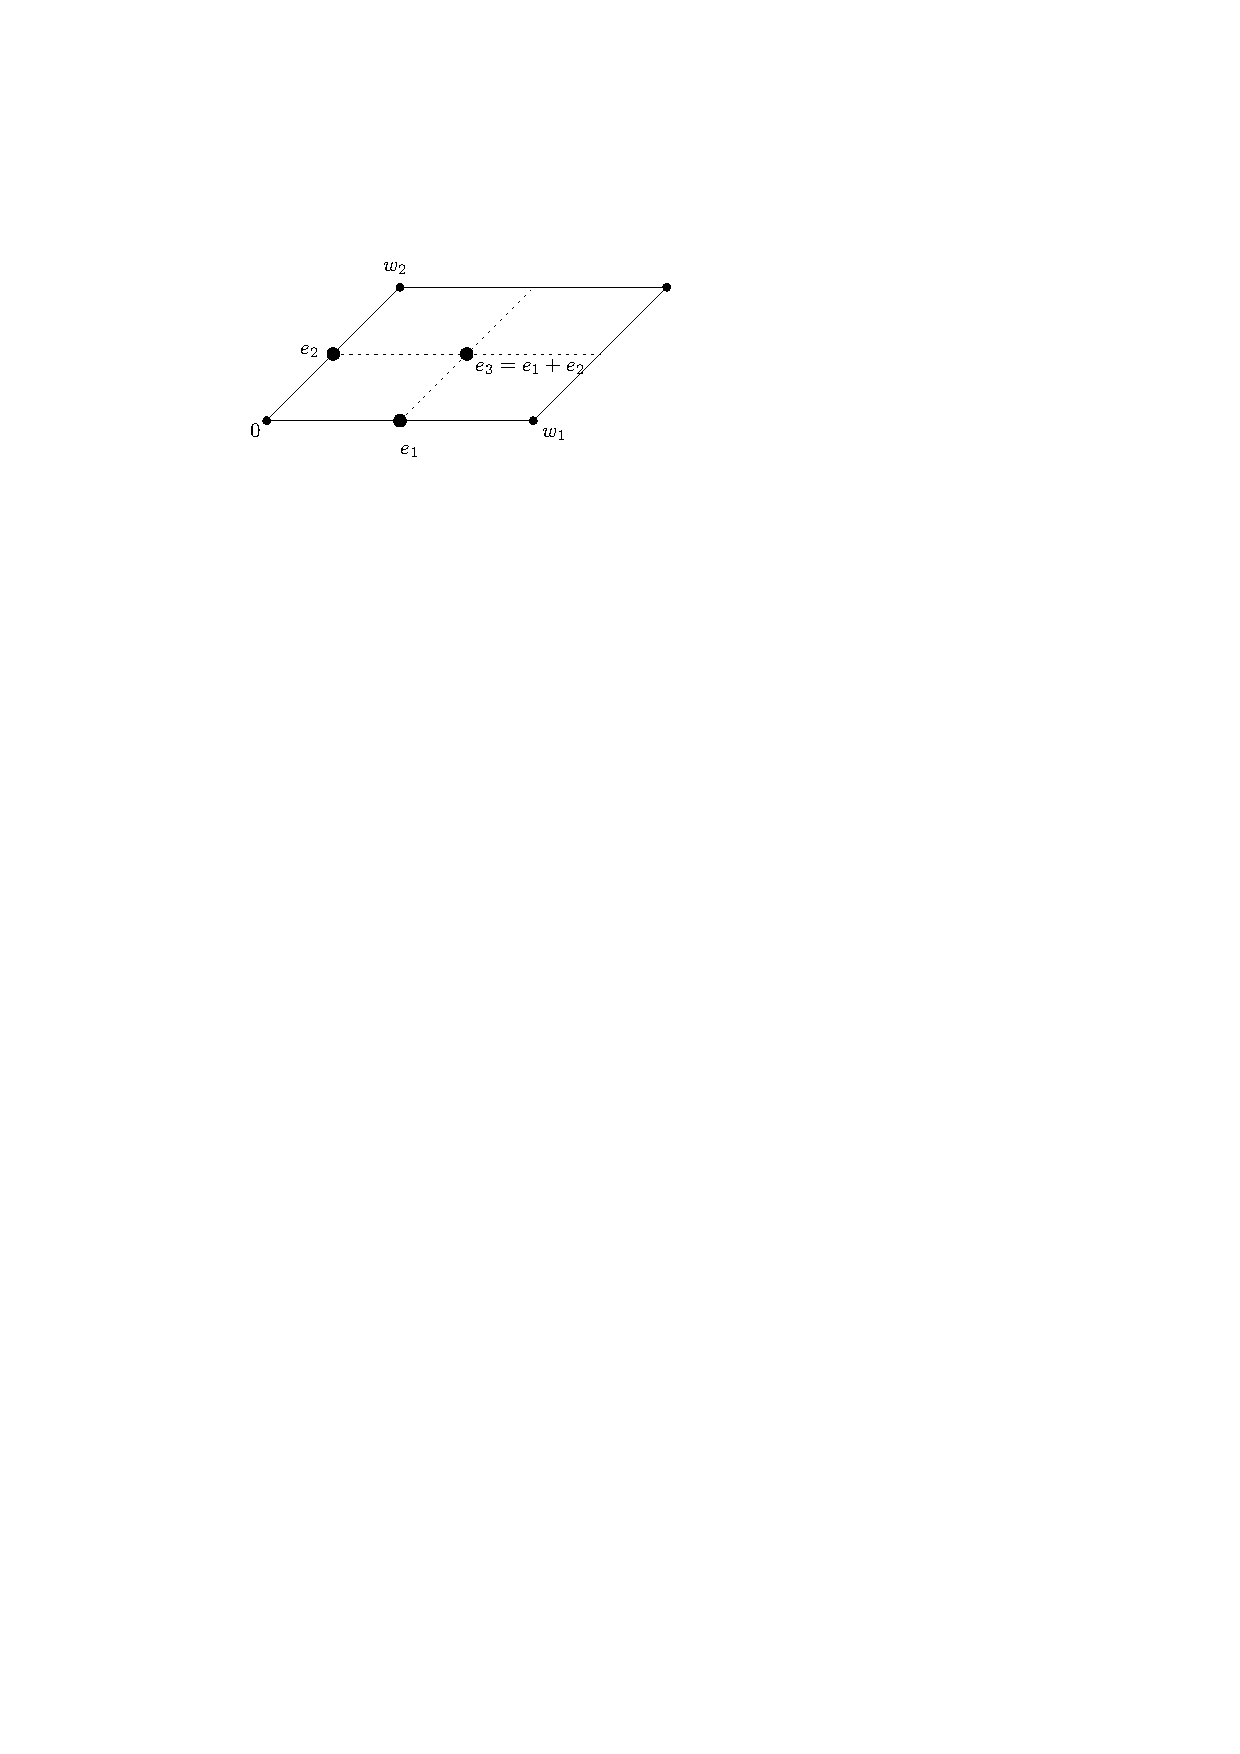
\includegraphics[height=2cm]{twotorsion.pdf}
  \caption{The $2$-torsion points of $E_\Lambda$}
  \label{fig:two-torsion}
\end{figure}

To summarize, what we have found is that there is a holomorphic map:
\[
\CC/\Lambda\to E_\Lambda,\quad z+\Lambda\mapsto (\wp_\Lambda(z),\wp_\Lambda'(z)),
\]
and this map is indeed a bijection: if $x\in\CC$ is any complex number, then $\wp_\Lambda$ takes the value $x$ twice, since $\wp_\Lambda(\pm z+\Lambda)=x$. Therefore we get two $y$-values unless $y=0$ (which happens only when $z=w_i/2$). In this case, $\wp_\Lambda(z)=e_i$, and $\wp_\Lambda(z)$ takes the value $e_i$ ``twice'' at $z$.

The following result is crucial:
\begin{theorem}[Uniformization theorem]
  If $E\colon Y^2=4X^3-g_2X-g_3$ is any elliptic curve, then there exists some lattice $\Lambda$ such that $g_2(\Lambda)=g_2$ and $g_4(\Lambda)=g_4$.
\end{theorem}
\begin{proof}
It uses that $j(z)$ is surjective. See~\cite[Proposition 1.4.3]{diamond-shurman}
\end{proof}
\begin{remark}
  \begin{enumerate}
  \item For $\tau\in\HH$, consider the elliptic curve $E_\tau=E_{\Lambda_\tau}$.
\[
E_\tau\colon Y^2=4X^3-g_2(\tau)X-g_3(\tau).
\]
One can compute that the discriminant of the cubic polynomial on $X$ that is the right-hand side is
\[
\tilde\Delta(\tau) = \frac{1}{16}(g_2(\tau)^3-27g_3(\tau)^2),
\]
which equals $\frac{(2\pi)^{12}}{16}\Delta(\tau)$,
where $\Delta(\tau)$ is the modular form already studied in Section~\ref{sec:a-product-formula-for-Delta}.
\item The map $\CC/\Lambda\to E_\Lambda$ is a group homomorphism. Or if we prefer, we may define the group structure on $E_\Lambda$ via transport of structure.
  \end{enumerate}
\end{remark}

\subsection{Moduli space interpretation}

Consider the set $S$ of isomorphism classes of elliptic curves. Every elliptic curve is isomorphic to $\CC/\Lambda$ for some lattice $\Lambda$, and in fact it is isomorphic to $\CC/\Lambda_\tau$ for some $\tau\in\HH$. Moreover,
\[
\CC/\Lambda_\tau\cong \CC/\Lambda_{\tau'}\iff \SL_2(\ZZ)\tau = \SL_2(\ZZ)\tau'.
\]
Therefore there is a natural bijection
\[
S\longleftrightarrow \SL_2(\ZZ)\backslash \HH,\quad [\CC/\Lambda_\tau]\mapsto \SL_2(\ZZ)\tau.
\]
The quotient $\SL_2(\ZZ)\backslash\HH$ is called the \emphh{moduli space} for isomorphism classes of elliptic curves.

Let now $f\in M_k(\SL_2(\ZZ))$ be a modular form of weight $k$. Define the following function $F$ on the set of complex tori:
\[
F(\CC/\Lambda_\tau) = f(\tau).
\]
This is well defined, because if $\Lambda_\tau=\Lambda_{\tau'}$ then $\tau=\tau'+b$ for some $b\in\ZZ$, and $f(\tau+b)=f(\tau)$. Moreover, suppose that $m\Lambda_\tau=\Lambda_{\tau'}$. Then
\[
\tau=\mtx abcd \tau',\quad m=c\tau'+d.
\]
Then we may compute:
\[
F(\CC/m\Lambda_\tau)=F(\CC/\Lambda_{\tau'}) = f(\tau')=(c\tau'+d)^{-k}f(\tau)=F(\CC/\Lambda_\tau)m^{-k}.
\]
From this we deduce that
\[
F(\CC/m\Lambda) = m^{-k}F(\CC/\Lambda).
\]
We could thus define modular forms as functions on complex tori satisfying the above relations. This prototype can be pushed to work for other congruence subgroups, although isomorphism classes of elliptic curves will have to be replaced by objects carrying more data.

\section{Moduli interpretation for \texorpdfstring{$\Gamma_0(N)$}{Gamma0(N)} and \texorpdfstring{$\Gamma_1(N)$}{Gamma1(N)}}
We will write $E[N]$ for the $N$-torsion in $E=\CC/\Lambda$, which is isomorphic to  $\ZZ/N\ZZ\times \ZZ/N\ZZ$.
\begin{figure}[h]
  \centering
  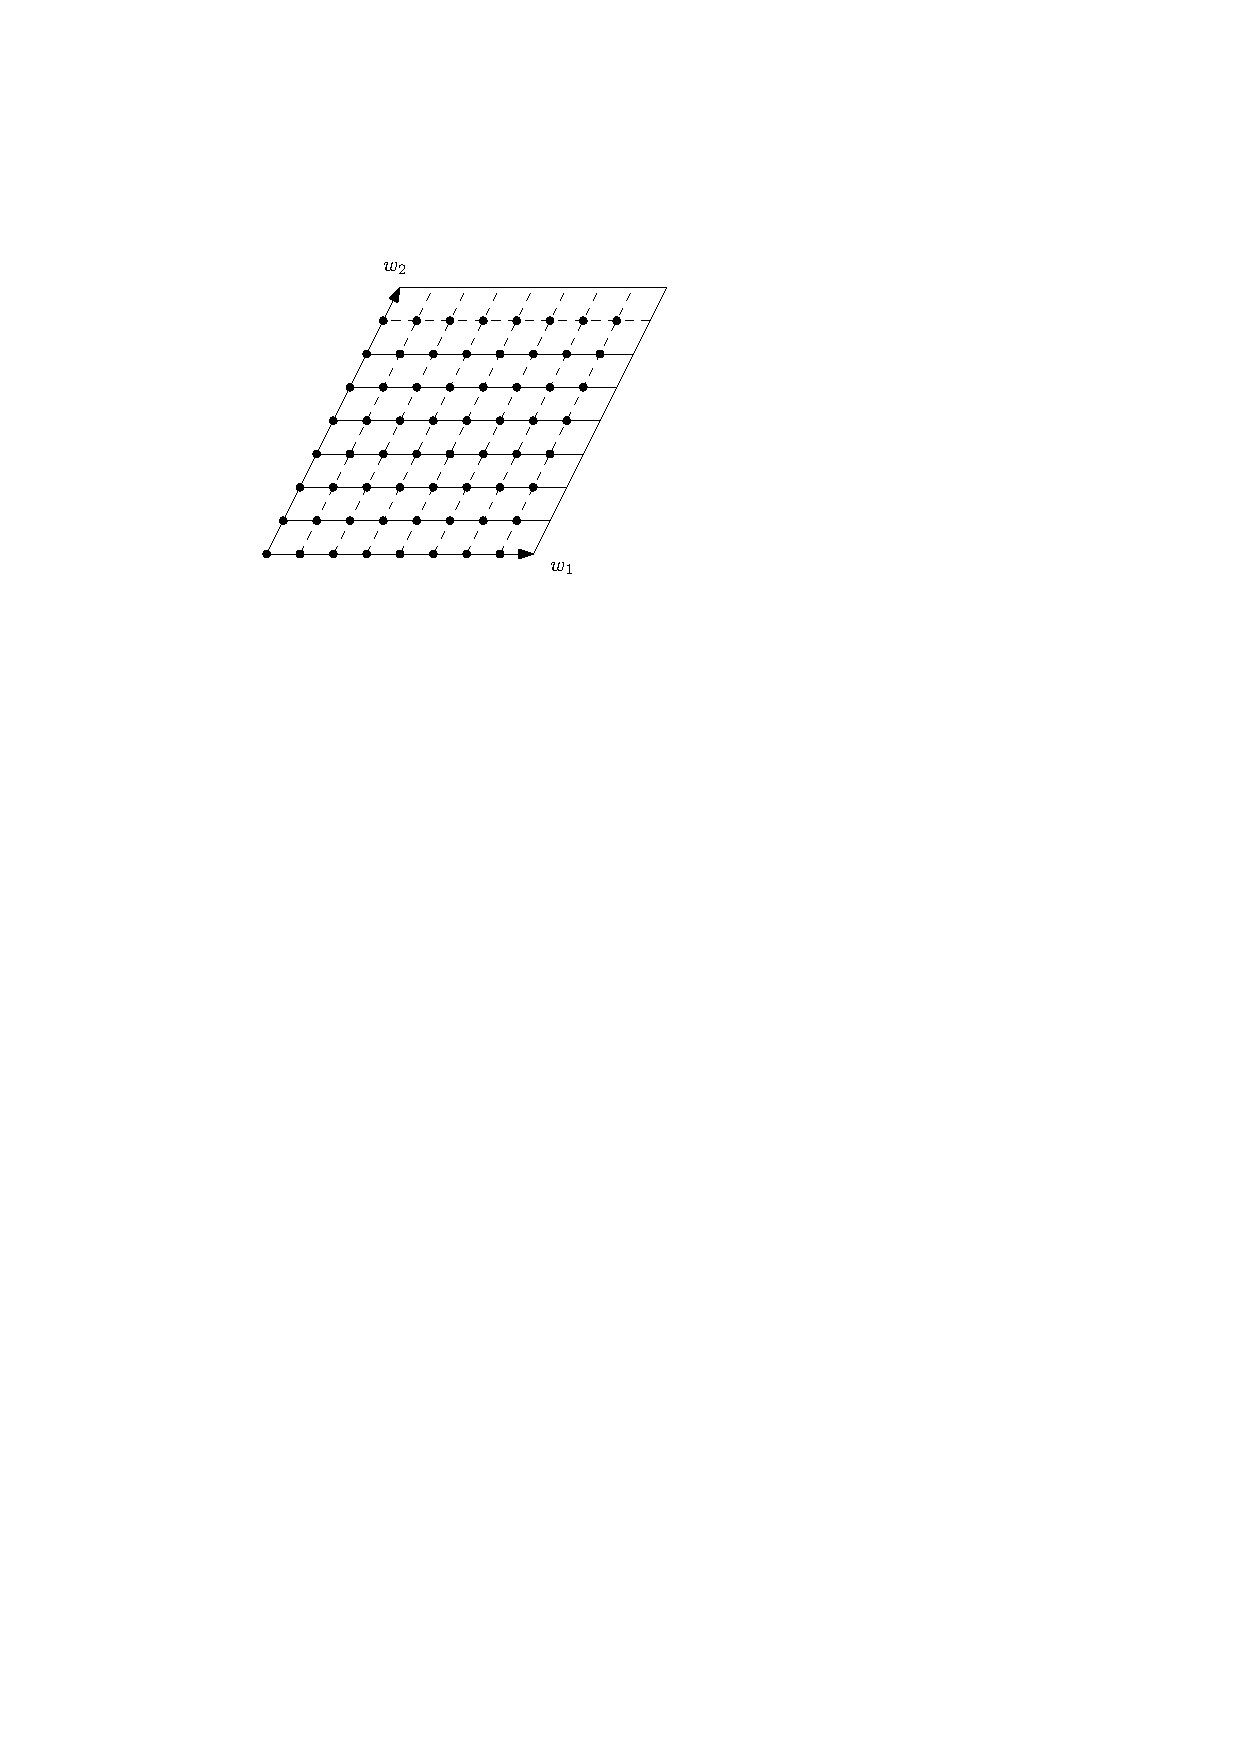
\includegraphics{ntorsion.pdf}
  \caption{The $8$-torsion of a complex torus $\CC/(\ZZ w_1 + \ZZ w_2)$.}
  \label{fig:n-torsion}
\end{figure}
In order to give a moduli interpretation for modular forms on $\Gamma_0(N)$, we need to add more structure
to the elliptic curves (or complex tori) that we consider.
\begin{definition}
  An \emphh{enhanced elliptic curve} for $\Gamma_0(N)$ is a pair $(E,C)$, where $E$ is an elliptic curve
and $C$ is a cyclic subgroup of order $N$ in $E[N]$. Two enhanced elliptic curves $(E,C)$ and $(E',C')$ are
equivalent if there exists an isomorphism $\varphi\colon E\tto{\simeq} E'$ such that $\varphi(C)=C'$.
\end{definition}
We write $S_0(N)$ for the set of equivalence classes of enhanced elliptic curves.

\begin{theorem}
  With the above notation,
  \begin{enumerate}
  \item Each class in $S_0(N)$ has a representative of the form $(\CC/\Lambda_\tau,\langle \frac{1}{N} + \Lambda_\tau\rangle)$, for some $\tau\in\HH$.
  \item Two pairs $(\CC/\Lambda_\tau,\langle \frac{1}{N}+\Lambda_\tau\rangle)$ and $(\CC/\Lambda_{\tau'},\langle \frac{1}{N}+\Lambda_{\tau'}\rangle)$ are equivalent if and only
if $\Gamma_0(N)\tau=\Gamma_0(N)\tau'$. Therefore the map $\tau\mapsto (\CC/\Lambda_\tau,\langle \frac 1N+\Lambda_\tau\rangle)$ induces a bijection of $Y_0(N)=\Gamma_0(N)\backslash\HH\cong S_0(N)$.
  \end{enumerate}
\end{theorem}

\begin{proof}
  Consider an enhanced elliptic curve $(\CC/\Lambda,C)$. We have already seen that there is an isomorphism $\varphi\colon\CC/\Lambda\cong \CC/\Lambda_{\tau'}$ for some $\tau'\in\HH$.
Since $C$ is cyclic of order $N$, the same is true for $\varphi(C)$. Therefore $(\CC/\Lambda,C)$ is equivalent to $(\CC/\Lambda_{\tau'},\langle\frac{c\tau'+d}{N}+\Lambda_{\tau'}\rangle)$ for some integers $c$ and $d$ coprime to each other
and to $N$. Since reduction modulo $N$ gives a surjection $\SL_2(\ZZ)\surjects \SL_2(\ZZ/N/ZZ)$, one can find a matrix
\[
\gamma=\mtx{a'}{b'}{c'}{d'}\in\SL_2(\ZZ),
\]
such that $c'\equiv c\pmod{N}$ and $d'\equiv d\pmod{N}$. Set now $\tau=\gamma\tau'$ and $m=c'\tau'+d'$, so $m\Lambda_\tau=\Lambda_{\tau'}$ and, as we wanted to show,
\[
m\left(\frac 1N + \Lambda_\tau\right)=\frac{c'\tau'+d'}{N}+\Lambda_{\tau'} = \frac{c\tau'+d}{N}+\Lambda_{\tau'},.
\]


As for the second part, for an isomorphism between $\CC/\Lambda_{\tau}$ and $\CC/\Lambda_{\tau'}$ to exist there needs to exist $\gamma=\smtx abcd\in\SL_2(\ZZ)$ such that
\[
(c\tau'+d)\Lambda_\tau = \Lambda_{\tau'}.
\]
Moreover, for the corresponding isomorphism to respect the cyclic subgroups one needs to have
\[
\langle(c\tau'+d)(\frac 1N+\Lambda_\tau)\rangle =\langle \frac 1N+\Lambda_{\tau'}\rangle.
\]
That is, $\gamma$ satisfies
\[
\langle\frac{c\tau'+d}{N}+\Lambda_{\tau'}\rangle = \langle\frac 1N+\Lambda_{\tau'}\rangle,
\]
which is equivalent to $N\mid c$ (and then $d$ is necessarily coprime to $N$). This last condition is precisely saying that $\gamma$ must belong to $\Gamma_0(N)$.
\end{proof}

In this context, one may define a weight-$k$ homogeneous function $F$ for $\Gamma_0(N)$ as a function on enhanced elliptic curves for $\Gamma_0(N)$ such that
\[
F((\CC/m\Lambda,mC) = m^{-k}F(\CC/\Lambda,C),\quad \forall m\in\CC.
\]
Given such an $F$, one can define $f(\tau)=F(\CC/\Lambda_\tau,\langle \frac 1N+\Lambda_\tau\rangle)$ and check that $f(\tau)$ is weakly modular of weight $k$ for $\Gamma_0(N)$.

We have a similar construction for $\Gamma_1(N)$.
\begin{definition}
  An \emphh{enhanced elliptic curve} for $\Gamma_1(N)$ is a pair $(E,P)$, where $E$ is an elliptic curve
and $P$ is a point of exact order $N$ in $E[N]$. Two enhanced elliptic curves $(E,P)$ and $(E',P')$ are
equivalent if there exists an isomorphism $\varphi\colon E\tto{\simeq} E'$ such that $\varphi(P)=P'$.
\end{definition}
We write $S_1(N)$ for the set of equivalence classes of enhanced elliptic curves for $\Gamma_1(N)$.

\begin{theorem}
  With the above notation,
  \begin{enumerate}
  \item Each class in $S_1(N)$ has a representative of the form $(\CC/\Lambda_\tau,\frac{1}{N} + \Lambda_\tau)$, for some $\tau\in\HH$.
  \item Two pairs $(\CC/\Lambda_\tau,\frac{1}{N}+\Lambda_\tau)$ and $(\CC/\Lambda_{\tau'}, \frac{1}{N}+\Lambda_{\tau'})$ are equivalent if and only
if $\Gamma_1(N)\tau=\Gamma_1(N)\tau'$. Therefore the map $\tau\mapsto (\CC/\Lambda_\tau, \frac 1N+\Lambda_\tau)$ induces a bijection of $Y_1(N)=\Gamma_1(N)\backslash\HH\cong S_1(N)$.
  \end{enumerate}
\end{theorem}
\begin{proof}
  Let $(E,Q)$ be any point in $S_1(N)$. Since $E$ is isomorphic to $\CC/\Lambda_{\tau'}$ for some $\tau'\in\HH$, we may take $E=\CC/\Lambda_{\tau'}$, and hence $Q=(c\tau'+d)/N + \Lambda_{\tau'}$ for some $c,d\in\ZZ$. The fact that the order of $Q$ is exactly $N$ means that $\gcd(c,d,N)=1$, and therefore there exists $a,b,k\in\ZZ$ such that
\[
ad-bc-kN=1.
\]
Note that this means that the matrix $\smtx abcd$ has determinant $1\pmod N$. Using that $\SL_2(\ZZ)$ surjects into $\SL_2(\ZZ/N\ZZ)$ and the fact that $c$ and $d$ only matter modulo $N$, we find a matrix $\gamma\in\SL_2(\ZZ)$ with lower low $(c,d)$. Let $\tau=\gamma\tau'$, and let $m=c\tau'+d$. Then we obtain $m\tau=a\tau'+b$, which implies that $m\Lambda_\tau = \Lambda_{\tau'}$. Moreover,
\[
m\left(1/N+\Lambda_\tau\right) = \frac{c\tau'+d}{N}+\Lambda_{\tau'} = Q.
\]
Therefore the class $[E,Q]$ is the same as $[\CC/\Lambda_\tau,1/N+\Lambda_\tau]$.

Finally, given two points $\tau,\tau'\in\HH$ such that $\Gamma_1(N)\tau=\Gamma_1(N)\tau'$, we may write $\tau=\gamma\tau'$ for some $\gamma=\smtx abcd\in\Gamma_1(N)$. Letting $m=c\tau'+d$, then:
\[
m\Lambda_\tau=\Lambda_{\tau'},\quad m\left(1/N+\Lambda_\tau\right)=\frac{c\tau'+d}{N}+\Lambda_{\tau'}.
\]
Since $(c,d)\equiv(0,1)\pmod N$, the last term is just $1/N+\Lambda_{\tau'}$, as we wanted to show.
\end{proof}
Moreover, note that there is a natural map $S_1(N)\to S_0(N)$, which sends the class of $(E,P)$ to that of $(E,\langle P\rangle)$.

There is a moduli space description of $\Gamma(N)\backslash\HH$ which classifies pairs of an elliptic curve $E$ with a \emph{basis} for $E[N]$, but its precise description requires the Weil pairing, which we have not seen in this course.

%%% Local Variables: 
%%% mode: latex
%%% TeX-master: "main"
%%% End: 
